%-----------------------------------------------
% Template para criação de relatórios de DAPI trabalho 3
% jlopes AT fe.up.pt,  Tue Dec 11 09:44:07 2007
%-----------------------------------------------

\documentclass[twocolumn,twoside,10pt,a4paper]{article}

%% packages
\usepackage[portuguese]{babel}    % português
\usepackage{graphicx}           % images .png or .pdf w/ pdflatex OR .eps w/ latex
\usepackage[T1]{fontenc}
\usepackage{lmodern}            % fonts
\usepackage[utf8]{inputenc}     % 8 bits 
\usepackage{indentfirst}        % more on tables
\usepackage{lastpage}           % to have lastpage in headers
\usepackage{url}                % URLs
%\usepackage[pagebackref]{hyperref} %hyper-refs and back refs

% page layout
\RequirePackage[outer=20mm,inner=30mm,vmargin=20mm,includehead,includefoot,headheight=15pt]{geometry}

%% space between columns
\columnsep 12mm

%% headers & footers
\usepackage{fancyhdr}
\pagestyle{fancy}
\fancyhead{}            % clear all fields
\fancyhead[LE,RO]{\emph{Análise e Preparação de Dados da BBC News}}
\fancyhead[RE,LO]{}
\fancyfoot{}            % clear all fields
\fancyfoot[C]{\textit{\thepage\ de \pageref{LastPage}}}
\fancyfoot[LE,RO]{\textit{DAPI, Grupo 2, \today}}
\renewcommand{\headrulewidth}{0pt}
\renewcommand{\footrulewidth}{0pt}
%\thispagestyle{plain}   % not in the 1st page
%% alternatively fancyplain could be used

% avoid widows and orphans
\clubpenalty=300
\widowpenalty=300

\title{Análise e Preparação de Dados da BBC News}

\author{Clara Sacramento\\
\footnotesize Faculdade de Engenharia da Universidade do Porto,\\[-0.8ex]
\footnotesize R.\ Dr.\ Roberto Frias, 4200-465 Porto\\[-0.8ex]
\small \texttt{ei09090@fe.up.pt}\\
\and
Diogo Teixeira\\
\footnotesize Faculdade de Engenharia da Universidade do Porto,\\[-0.8ex]
\footnotesize R.\ Dr.\ Roberto Frias, 4200-465 Porto\\[-0.8ex]
\small \texttt{ei09086@fe.up.pt}\\
}

\begin{document}

\maketitle

\selectlanguage{portuguese}
\begin{abstract}

A \textit{BBC} é uma das maiores cadeias de media a nível mundial. Entre as suas variadas divisões encontra-se a \textit{BBC News}, uma das mais importantes e prestigiadas agências noticiosas do mundo. No entanto, os serviços de pesquisa sobre os seus vastos repositórios de notícias são simplistas, e pouco personalizáveis. Pretende-se assim fazer um estudo sobre novas funcionalidades que possam ser adicionadas ao serviço, de forma a melhorar a experiência dos utilizadores. Consequentemente será também construído um repositório \textit{offline} de notícias.

\end{abstract}

\section{Introdução}\label{sec:intro}

Este documento descreve de uma forma sintética o trabalho de escolha, análise e caracterização de um conjunto de dados, feito até ao momento da sua escrita. Neste trabalho foram analisadas grandes quantidades de notícias, extraídas a partir das plataformas \textit{web} da \textit{BBC News}. Pretende-se que com base nesta análise seja possível desenvolver novas funcionalidades de pesquisa e apresentação de conteúdos, melhorando assim a experiência dos utilizadores destas plataformas.

A Secção 2 está reservada a uma breve exposição dos fatores considerados para garantir a qualidade do conjunto de dados utilizados. Na Secção 3 é apresentado o modelo conceptual que representa a organização dos dados obtidos. Mais à frente, nas Secções 4 e 5, é feita uma análise mais detalhada e técnica sobre a obtenção, processamento e armazenamento de dados. Na Secção 6 são analisadas possíveis tarefas de pesquisa a efetuar. Por fim, na Secção 7, são apresentadas as conclusões deste documento.

\section{Qualidade dos Dados}\label{sec:quality}

O conjunto de dados usado será diretamente extraído de páginas \textit{web} sob a alçada da \textit{BBC News}. Uma vez que o conteúdo destas páginas é controlado na totalidade por esta última agência noticiosa, a qualidade, bem como a fiabilidade dos dados está assegurada.

É ainda importante referir a qualidade dos suportes nos quais os dados são disponibilizados, uma vez que a obtenção destes dados é feita sobretudo através de \textit{screen scraping} de páginas \textit{web}. Nos casos analisados até à altura de escrita deste relatório, verifica-se que os suportes disponibilizados pela \textit{BBC News} são consistentes, e principalmente bem estruturados. Isto significa que o processo de extração de dados pode ser facilmente automatizado definindo um número reduzido de regras de extração.

\section{Modelo Conceptual de Domínio}\label{sec:model}

A unidade de dados usada no domínio deste serviço é a notícia. Uma notícia inclui os seguintes atributos: id, título, descrição, o corpo da notícia, a data de publicação, e o endereço de consulta na página da \textit{BBC News}. Existem outros atributos adicionais de uma notícia, nomeadamente o número de vezes que a notícia foi partilhada nas redes sociais e a indicação se a notícia contém conteúdo áudio e/ou vídeo. É possível que em versões posteriores as notícias possam incluir novos atributos (ver Figura \ref{fig:domain}).

\begin{figure}[ht]
\centerline{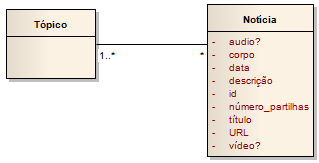
\includegraphics[width=0.4\textwidth]{domain.png}}
\caption{{\it Modelo conceptual de domínio.}}  
\label{fig:domain}
\end{figure}

O modelo conceptual de domínio conta ainda com a noção de tópico. Um tópico representa um aglomerado de notícias que partilham uma temática. Assim sendo, um tópico pode ter inúmeras notícias a si associadas. Uma notícia pode também estar associada a mais do que um tópico.

\section{Obtenção e Processamento dos Dados}\label{sec:processing}

A obtenção de notícias da \textit{BBC News} divide-se em três passos principais: interrogação à \textit{API} disponibilizada, obtenção das páginas \textit{web} de cada notícia, e processamento dessas páginas.
A \textit{BBC News} disponibiliza uma \textit{API} de acesso às notícias mais recentes. É uma \textit{API} simples, contando apenas com dois tipos de pedido \textit{REST}, maioritariamente usada como suporte a serviços \textit{RSS}. A aplicação de extração de dados desenvolvida obtém, através desta \textit{API}, a lista de todas as categorias de notícia disponíveis, em formato \textit{JSON}. Obtida e interpretada esta lista de categorias, é então possível executar um novo pedido à \textit{API}, que retorna um vetor de notícias. Cada notícia contém título, uma breve descrição, endereço de consulta, data de publicação e imagem \textit{thumbnail}.

A informação obtida através da \textit{API} é importante, mas muito incompleta. Como solução a este problema, é obtida a página \textit{web} correspondente a cada notícia no vetor previamente mencionado. Devido ao elevado número de pedidos e ao consequentemente elevado tempo de resposta, esta porção do processo foi paralelizada, de forma a reduzir o tempo de espera na obtenção dos dados.

Por fim, cada uma das páginas \textit{web} é processada, recorrendo a várias tecnologias de pesquisa sobre documentos (seletores \textit{CSS}, seletores \textit{XPath} e expressões regulares). Este processamento permite não só obter o corpo de cada notícia, como também enriquecer cada uma com novas informações. Como exemplo de informações adicionais temos o grau de popularidade de cada notícia, ou a sinalização de conteúdos vídeo/áudio.

\section{Armazenamento dos Dados}\label{sec:store}

O processamento e obtenção de dados da \textit{BBC News}, realizado com frequência diária, produz grandes quantidades de informação. A técnica de \textit{screen scraping} exige uma calibração cuidadosa nesta fase inicial do trabalho, muitas vezes conseguida através da análise manual dos resultados obtidos. Assim sendo, torna-se importante armazenar a informação num formato estruturado, que possa ser facilmente entendido e analisado, tendo-se optado neste caso pelo formato \textit{XML} (ver Figura \ref{fig:xml}).

Em versões posteriores da aplicação de extração de dados estes serão armazenados em bases de dados relacionais. Esta mudança tem como objetivos facilitar a consulta da informação através de interrogações em \textit{SQL}, e proporcionar o armazenamento da informação de uma forma centralizada. Será também implementado um conversor que permitirá transferir toda a informação armazenada nos ficheiros \textit{XML} para uma base de dados relacional, de forma automática.

\begin{figure*}[ht]
\centering
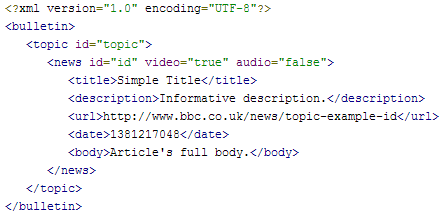
\includegraphics[width=0.6\textwidth]{xml.png}
\caption{\it Estrutura típica de armazenamento dos dados.}
\label{fig:xml}
\end{figure*}

\section{Tarefas de Pesquisa Consideradas}\label{sec:work}

Para este trabalho foram consideradas quatro grandes vertentes de pesquisa sobre o conjunto de dados estudado: pesquisa textual simples, pesquisa por imagem, refinamento de pesquisa e organização de resultados.

A pesquisa textual consiste simplesmente na busca de uma ou várias palavras no texto indexado, nomeadamente no título, descrição ou corpo da notícia. Esta é a pesquisa mais comum, e está já disponível através das plataformas da \textit{BBC News}.

Foi também estudada a possibilidade de utilizar pesquisa por imagem, quer por comparação direta entre imagens, quer por indexação de atributos de imagens através do modelo \textit{bag-of-words} \cite{wiki:bow}. Esta opção foi no entanto posta de parte, uma vez que requer um grande esforço de implementação, muito para além do domínio deste trabalho.
Um dos pontos principais do trabalho é a possibilidade de refinar a pesquisa textual através de vários atributos. Até este momento foi estudada a filtragem por data de publicação, por tópico, por exclusão de campos usados para pesquisa textual e por artigos com conteúdos áudio e/ou vídeo.

Por fim, foram ainda estudadas possibilidades de ordenação de resultados. Para além da ordenação por data, será possível a organização por “popularidade”, sendo que um artigo é tanto mais popular quantas mais vezes for partilhado nas redes sociais. 

Mais tarde, com posterior análise às páginas web obtidas, poderá ser possível encontrar novos métodos de organização ou refinamento de pesquisas.

\section{Conclusões}\label{sec:conclude}

\bibliographystyle{unsrt}
\bibliography{biblio}

\end{document}
